%!TEX root = report.tex

\section{Methods}\label{sec:methods}

\subsection{Environment}\label{sec:environment}
\begin{figure}[h]
    \centering
    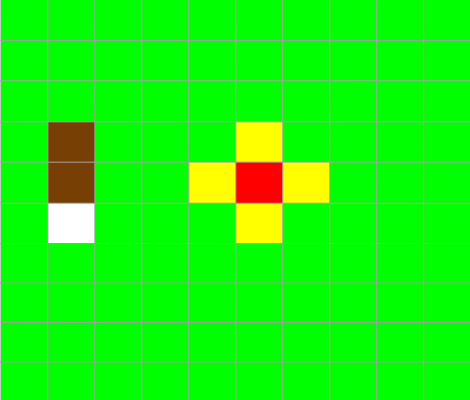
\includegraphics[width=\linewidth]{img/Simulation.png}
    \caption{A visual representation of the environment. The agent is shown in white, leaving behind a trail of inflammable dug cells (shown in brown). The trees (green) can ignite to become burning cells (red), which heat up the neighbouring cells (yellow). When a burning cell runs out of fuel it dies (black)}
    \label{fig:simulation}
\end{figure}
The forest fire is simulated using a grid of cells, each of which has a number of attributes. The main ones are heat potential, temperature, ignition threshold and fuel. Heat potential is the amount of heat, once ignited, the cell radiates to its neighbours to increase their temperature. As soon as the temperature of a cell reaches the ignition threshold, the cell ignites and burns. A burning cell consumes one fuel per iteration, and stops burning and radiating heat when the fuel is empty, becoming a dead cell. The heat from a burning cell reaches the cells directly north, south, east and west of it. If that cell is flammable its temperature is increased by the heat potential of the burning cell, otherwise nothing happens.

For a visual representation please see Figure \ref{fig:simulation}. The shape of the grid is always square and has a size of either 10-by-10 or 14-by-14 cells. The green cells represent trees that can be ignited. The agent (or bulldozer) is represented by the white tile. Wherever it moves it destroys the trees and an empty, inflammable (brown) cell is formed. A line of these dug cells forms a fire line over which the fire cannot spread. Dead cells are represented in black. The agent has to move each time step, it is not allowed to idle on the same cell, and it can only die if it moves into an actively burning (red) cell. The only possible actions for the agent to take are the 4 valid movements (north, south, east, west), and the agent is always digging as it moves. The environment reaches a terminal state and restarts if the agent dies, or if there are no more burning cells.

\subsubsection{The Reward Function}\label{sec:reward_function}
Any reinforcement learning algorithm will rely on the two things that constitute the input to the agent. The quality of the state representation, or in other words how much of- and how well the agent can perceive the environment, and the quality of the reward function, which defines how well the agent's notion of success corresponds with the desired behaviour. Because of this, the performance of the agent may depend heavily on the design of the reward function.

The reward function also determines the speed at which the agent will be able to learn the optimal policy. To take the gradient descent analogy of a problem landscape, if the reward function produces a smooth gradient to the optimal solution, the agent will be able to find a path to that solution more easily than if the reward resembles a flat landscape with sparse spikes in which the value jumps from almost always 0 or negative to a positive reward \citep{sutton_barto_2018}. In other words, the agent should be provided gradual feedback instead of sparse and delayed rewards in order to facilitate fast and efficient learning. 

We defined the reward function as
\begin{equation}\label{eq:reward_function}
    R_t = \left\{\begin{array}{lr}
        1000, & \text{ Fire is contained }\\
        1000 * (p), & \text{ Fire burns out }\\
        -1000, & \text{ Agent dies }\\
        -1, & \text{ Otherwise }

        \end{array}\right\},
\end{equation}
where $p$ is the percent of the map undamaged by either fire or digging. Note that this reward function does not produce a smooth gradient, and the performance of the agent will likely suffer as a result.

Containment of the fire is defined as
\begin{equation}\label{eq:containment}
    \sum_{f \in \mathcal{F}} \sum_{b \in \mathcal{B}} astar(f, b) = 0,
\end{equation}
where $f$ is a burning cell from the set of currently burning cells $\mathcal{F}$ and $b$ is a cell on the border of the map from the fixed set of border cells $\mathcal{B}$. The function $astar$ is defined as
\begin{equation}\label{eq:astar}
    astar(f, b) = \left\{
        \begin{array}{lr}
            1, & \text{ if A* path exists }\\
            0, & \text{ Otherwise }
        \end{array}\right\},
\end{equation}
where a path is a sequence of directly connecting cells starting with cell $f$ and ending with cell $b$, determined using the A* path-finding algorithm and not allowing diagonal steps. The intuition is that if there exists a path between any burning cell and any cell on the border of the map, then there exists a way for the fire to spread beyond control and so it is not contained.


\subsubsection{The State Representation}\label{sec:state_rep}
The state of the environment, as it is visible to the agent, consists of 3 matrices of size $N^2$ with a boolean domain resulting in, after flattening, an array of $3 * N^2$ boolean inputs where $N$ is the size of the square map. The environment is thus represented three times: One layer contains only the agent position, translating to a matrix of zeros except for a single one representing the position of the agent. The second layer consists of the positions of the fire. Cells that are on fire are represented by a 1, the rest are set to 0. The third layer represents the fire lines cut by the agent in a similar boolean fashion, resulting in a total of 300 inputs to the agent when $N=10$. This is shown graphically in Figure \ref{fig:visiongrid}.

\begin{figure}[h]
    \centering
    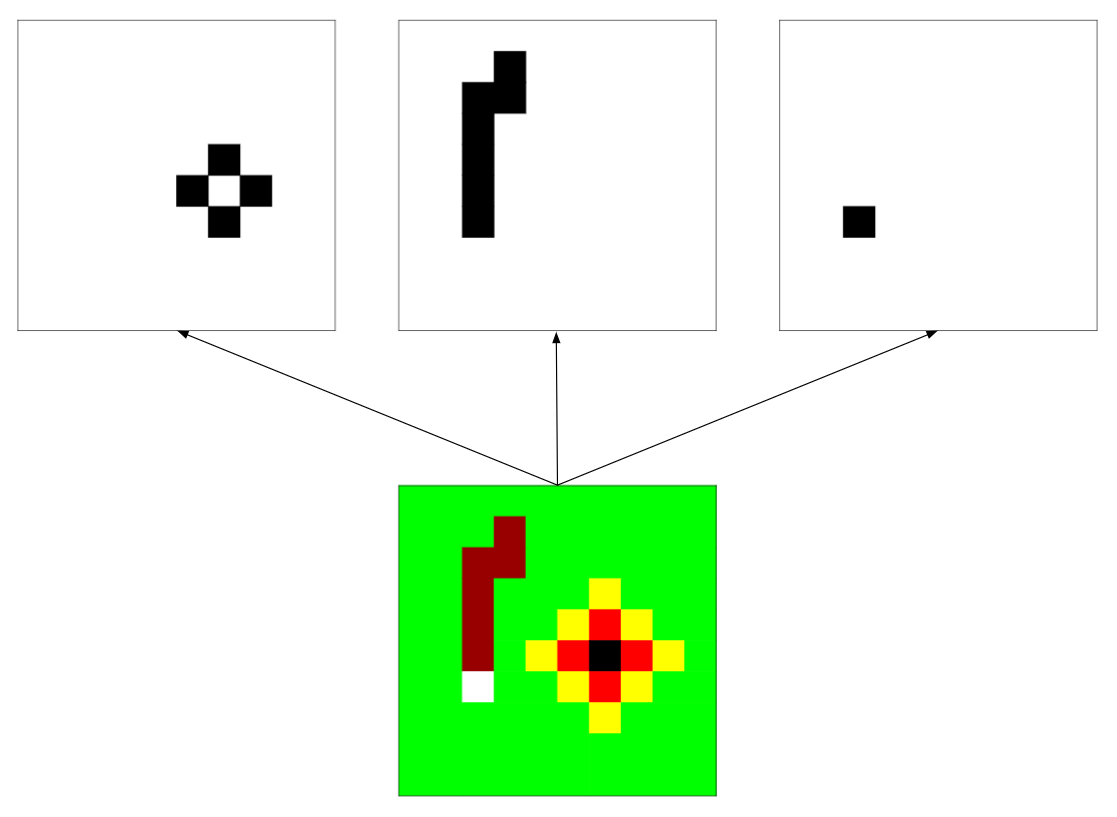
\includegraphics[width=1\linewidth]{img/State_Representation.png}
    \caption{An example of the state representation. Each layer shows an important aspect of the world: The location of the agent, the fire and of inflammable cells.}
    \label{fig:visiongrid}
\end{figure}

This state representation can speed up the learning process as well as increase performance \citep{knegt2018opponent}. Indeed it had a noticeable effect on the performance and learning speed of our implementation compared to a single matrix representing the gray-scaled map as input, likely because the agent can more easily differentiate between important attributes due to the boolean domain, and because only the relevant information is presented. Furthermore, the agent can now see whether the cell it is occupying is already dug or not.


\subsection{RL Algorithm}\label{sec:agent}

\subsubsection{Known Problems with Connectionist RL}\label{sec:problems}
The combination of function approximation (the neural network), bootstrapping (TD methods that update $Q$-values using estimated return values) and off-policy training (the $Q$-Learning algorithm) make up the deadly triad \citep{sutton_barto_2018}, which is known to cause instabilities and even divergence in the learning process. This is at least partly due to correlations in the sequence of consecutive observations, the fact that even small updates to $Q$ can change the policy and therefore the data distribution, and the correlations between the $Q$-values $Q(s_t, a_t; \theta_t)$ and the target values $Y_t = r_{t+1} + \gamma \max_a Q(s_{t+1}, a; \theta_t)$ \citep{mnih2015human}.

As will be clear by the end of this section, all three of these elements of the deadly triad are present in some of the algorithms. There are, however, two well known strategies to reduce this effect and stabilise learning: Using experience replay and a target network.

\subsubsection{Network Architecture}\label{sec:architecture}
First we define the neural network architecture\footnote{The source code is available at https://github.com/dashdeckers/Wildfire-Control-Python and can be accessed and used for non-commercial uses only.} that will approximate $Q$, or the action-value function. We use only a shallow network with one hidden layer of 50 units using a sigmoidal activation function, and a simple output layer with a linear activation. The network takes as an input a state $s$, consisting of an array of size $3*N^2$, and outputs an array of size 4 corresponding to the $Q$-values of taking any of the 4 possible actions $a$ in that state. We used the Adam optimizer to train this network.

\subsubsection{Experience Replay}\label{sec:exp_replay}
\begin{figure}[h]
    \centering
    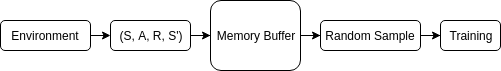
\includegraphics[width=1\linewidth]{img/Experience_Replay.png}
    \caption{Schematic structure of the experience replay process}
    \label{fig:expreplay}
\end{figure}
Instead of training the network on incoming experiences $e_t=(s_t,a_t,r_t,s_{t+1})$ at each time step $t$ directly, the experiences can be stored in a memory buffer $B_t=\{e_1,...e_t\}$ and the network can be trained on a mini-batch of memories randomly sampled from this buffer $(s,a,r,s') \sim U(B)$ (see Figure \ref{fig:expreplay}). The buffer $B$ allows for $M$ experiences to be stored until it is full, at which point the oldest memories will be discarded to make room for new ones.

This helps because neural networks assume that each training sample is identically and independently distributed from the population, which is in this case the set of $Q$-values that the network is set up to approximate, and training directly on incoming experiences violates this assumption in two regards.

For one, consecutive incoming experiences are obviously highly correlated because the environment does not radically change after any action (unless it is a terminal state). This means that any experience differs from the previous experience only to the extent to which the environment can change in one update step from a single action from the agent.

Secondly, the distribution of incoming experiences is also dependent on the agent's current policy. If the current policy determines that the agent should head east, then the next experiences recorded by the agent will involve the agent headed east. Apart from the obvious correlation, this can also lead to feedback loops and the network parameters could get stuck in local optima or even diverge \citep{tsitsiklis1997analysis,mnih2015human}.

In addition to stabilising the learning process, this approach also increases sample efficiency by allowing memories to be re-used multiple times until they are discarded when they reach the end of the queue. We can also pre-initialize this buffer with memories before learning to provide the agent with demonstration data, as will be explained in Section \ref{sec:demo_data}.


\subsubsection{Target Network}\label{sec:target_network}
Another source of instability arises when we use the predictions of the network to generate the target values which directly update the weights of that same network, as in the standard $Q$-learning update
\begin{equation}\label{eq:update_rule}
    \theta_{t+1} = \theta_t + \alpha(Y_t - Q(s_t, a_t; \theta_t))\nabla_{\theta_t}Q(s_t, a_t; \theta_t),
\end{equation}
where $\alpha$ is the learning rate and the target $Y_t$ is defined as
\begin{equation}\label{eq:target}
    Y_t \equiv r_t + \gamma \max_a Q(s_{t+1}, a; \theta_t).
\end{equation}

The update rule in \eqref{eq:update_rule} resembles stochastic gradient descent, updating the value $Q(s_t, a_t; \theta_t)$ towards the target value $Y_t$. Using the same network can lead to unwanted feedback loops. A delay to the loop can be added to reduce these effects by using a periodically updated, frozen copy of the network with weights $\theta^-$ to generate the target values instead (as shown schematically in Figure \ref{fig:targetnet})
\begin{equation}\label{eq:target_target}
    Y^{Target}_t \equiv r_{t+1} + \gamma \max_a Q(s_{t+1}, a; \theta_t^-),
\end{equation}
where every $C$ time steps, the weights of the network are copied into the target network $\theta_t^- = \theta_t$. This modification was also used by \cite{mnih2015human} alongside experience replay to make the algorithm more stable and dramatically increase its performance.

\begin{figure}[h]
    \centering
    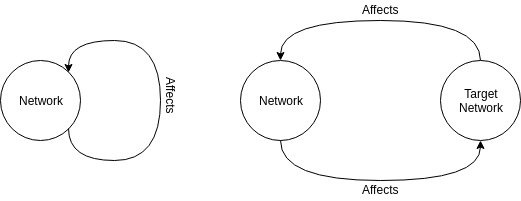
\includegraphics[width=1\linewidth]{img/Target_Network.png}
    \caption{Using a target network to add a delay to the feedback loop. The main network affects (copies itself into) the target network only every $C$ iterations.}
    \label{fig:targetnet}
\end{figure}


\subsubsection{Q-Learning versus SARSA}\label{sec:ql_sarsa}
We implemented both $Q$-Learning \citep{watkins1989learning} and SARSA \citep{rummery1994line} to investigate the difference in performance when using an off-policy versus on-policy algorithm. 

There are two commonly used policies, the greedy and the $\epsilon$-greedy policy, and both depend on $Q$. The greedy policy simply always chooses the best action to take in the current state at any given time step: $\argmax_a Q(s_t, a)$.

The $\epsilon$-greedy policy is similar, but it regulates the exploration/exploitation trade-off with the parameter $\epsilon \in [0,1]$. With a probability of $\epsilon$, this policy chooses a random action and otherwise chooses the best action. By annealing this probability towards 0 over time, we can ensure a high exploration rate in the beginning and then slowly decrease it to switch focus to the exploitation stage.

In $Q$-learning the agent follows the $\epsilon$-greedy policy while optimizing the greedy policy, making it an off-policy algorithm. Putting together everything so far, we end up with the following loss function for the base $Q$-Network algorithm:
\begin{equation}
    L_i(\theta_i)= \sum_{(s,a,r,s') \sim U(B)}[(Y^{Target}-Q(s,a,\theta_i))^2].
\end{equation}
Where $Y^{Target}$ is the target value defined in Equation \eqref{eq:target_target}.

In SARSA however, as the acronym suggests, we also save the next action to the memory buffer with the tuple $(s,a,r,s',a')$. This way the agent can both follow and optimize for the same $\epsilon$-greedy policy, making this an on-policy algorithm with the loss function:
\begin{equation}
    L_i(\theta_i)= \sum_{(s,a,r,s',a') \sim U(B)}[(Y^{SARSA}-Q(s,a,\theta_i))^2].
\end{equation}
with
\begin{equation}\label{eq:target_sarsa}
    Y^{SARSA}_t \equiv r_{t+1} + \gamma Q(s_{t+1}, a_{t+1}; \theta_t^-).
\end{equation}
This should lead to an increase in learning stability due to one less element of the deadly triad present in the system. Because SARSA updates $Q$ in a way that takes into account the random actions the agent sometimes takes it is expected to find a safer, but less optimal policy \citep{sutton_barto_2018} and report a higher average performance during learning.


\subsubsection{Dueling Networks}\label{sec:dueling}
One limitation of the $Q$-Network approach is that it is not able to estimate the value of a state and the action separately \citep{wang2015dueling}. This ability can be very useful, since often in states an action has no relevant consequence. The dueling network architecture achieves this by having two streams each predicting different things, instead of one stream predicting both. It is implemented by configuring two hidden layers in parallel, replacing the single hidden layer that is standard in the Q-Network. One of these two layers will estimate the state value $V$, while the other layer will estimate the action advantages $A$ for all possible actions. The two are merged together according to Equation \eqref{eq:dueling}. This equation differs from the original paper, since here we do not use any convolutional layers.

\begin{equation} \label{eq:dueling}
  \begin{array}{l}
    Q(s,a; \alpha, \beta) = V(s; \beta) + \\ 
    \Big(A(s, a; \alpha) - \frac{1}{c} \sum\limits_{a'} A(s,a'; \alpha)\Big)
  \end{array}
\end{equation}

Here, $\alpha$ and $\beta$ denote the weights of the two fully connected layers and $c$ the number of actions. This equation automatically prevents the layer for the state value from estimating anything related to the action advantages, since the sum of the advantages is kept at zero. The equation results in the $Q$-values which can be used in the same way as the single stream Q-values. All learning techniques and code can be recycled, and the target network and experience replay is also used. Given the results from the original paper, this modification is expected to boost the maximum performance and especially the speed of learning. 

\subsubsection{Dueling SARSA}\label{sec:duelingsarsa}
As well as combining dueling networks with $Q$-Learning, we also combine on-policy SARSA with the dueling network architecture to introduce a new RL algorithm, Dueling SARSA. We expect this algorithm to benefit from both modifications for a twice improved performance and both increased learning speed and learning stability. Just as the other three algorithms, Dueling SARSA also uses the target network and experience replay.


\subsubsection{Demonstration Data}\label{sec:demo_data}
Because the reward function defined in Section \ref{sec:reward_function} provides only sparse and delayed rewards, the agent might require additional guidance to learn to contain the fire in a reasonable training time. To point it in the right direction, we can fill the memory buffer with demonstration data before learning as mentioned in Section \ref{sec:exp_replay}. The agent can then use these memories during the learning process to its advantage.

The demonstration data only needs to show the agent how it might be able to collect the containment reward, to this effect we developed a simple algorithm that moves the agent around the fire in a clockwise direction. It does this by choosing randomly from one of two possible actions, unless one of the actions would lead to the death of the agent in which case it chooses the safe action. The two possible actions depend on the position of the agent relative to the fire (This is shown schematically in Figure \ref{fig:demodata}).

The environment is reset upon containment as defined in Equation \eqref{eq:containment}. Only memories (transitions) leading to successful containments are stored. This results in an average of 35 memories per episode, or containments of the fire, on the 10x10 map, and around 48 memories per episode on the 14x14 map. The number of episodes of demonstration data required can be specified.

\begin{figure}[h]
    \centering
    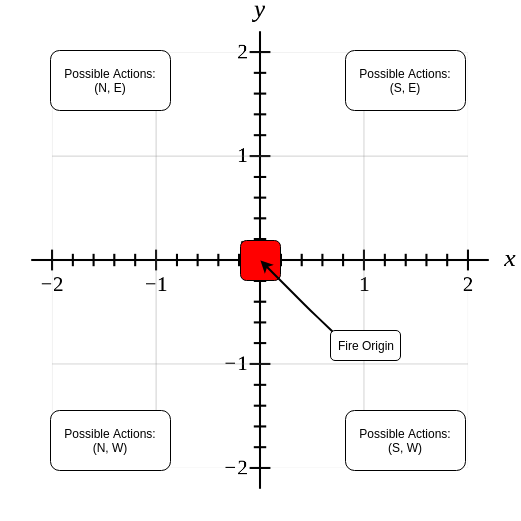
\includegraphics[width=1\linewidth]{img/Demo-data_Baseline.png}
    \caption{The possible actions for the agent to take, based on the position (quadrant) of the agent relative to the origin of the fire}
    \label{fig:demodata}
\end{figure}



\subsection{Experimental Setup}\label{sec:experiment}

\subsubsection{Baseline Algorithm}\label{sec:baseline}
To be able to reliably compare the performance of the different algorithms, we need a stable baseline. We build on the ideas discussed in Section \ref{sec:demo_data} to define the algorithm shown in Algorithm \ref{alg:baseline}. This algorithm is identical to the demonstration data generation except that it continues until the fire has burnt out, so it does not stop as soon as the fire is contained.

\begin{algorithm}
  \caption{Baseline algorithm to contain the fire}
  \label{alg:baseline}
  \begin{algorithmic}[1]
    \Procedure{RunBaseline}{}
    \State {totalreward = 0}
    \While {\textbf{not} done}
    \State {action = random(possible actions)}
    \If {action is dangerous}
    \State {action = other possible action}
    \EndIf
    \State {reward, done = execute(action)}
    \State {totalreward = totalreward + reward}
    \EndWhile
    \State \Return {totalreward}
    \EndProcedure
  \end{algorithmic}
\end{algorithm}

\subsubsection{Collection of Results}\label{sec:datacollection}
We investigate the performance of both $Q$-Learning and SARSA, both with and without the dueling network architecture modification, for a total of 4 different algorithms. The hyper-parameters we used throughout all experiments are shown in Table \ref{tab:hyperparameters}.

Each algorithm and parameter combination was run 10 times for 10,000 episodes per run. We compared the baseline performance to 2 map sizes ($N=10$ and $N=14$), 3 different amounts of demonstration data (0, 100 and 1000 episodes) and 4 algorithms for a total of 240 runs (260 including the baselines). At the start of each run, the environment is initialized with trees and a single cell at the center of the map is ignited. The agent starts at a random location on a circle centered around the fire with a radius of either 1, 2 or 3 (also randomly selected). Since each run took approximately 4.5 hours on average, they were calculated on the Peregrine computing cluster provided by the University of Groningen.

\begin{table}[H]
\centering
\begin{tabular}{|l|l|}
\hline
Memory size & 20000 \\ \hline
Batch size & 32 \\ \hline
Target update ($C$) & 20 \\ \hline
Gamma ($\gamma$) & 0.999 \\ \hline
Alpha ($\alpha$) & 0.005 \\ \hline
Epsilon decay ($\epsilon$) & 0.01 \\ \hline
Epsilon maximum & 1 \\ \hline
Epsilon minimum & 0.005 \\ \hline
\end{tabular}
\caption{All relevant hyper-parameters used in the training process. These values were selected by performing an informal search using the Q-Learning algorithm without dueling networks. The target is updated every $C$ episodes. The epsilon value is decayed after every episode.}
\label{tab:hyperparameters}
\end{table}
